\documentclass{article}
\usepackage[utf8]{inputenc}
\usepackage[margin=0.5in]{geometry}
\usepackage[portuguese]{babel}
\usepackage{graphicx}
\usepackage{amsmath}
\graphicspath{ {./images/} }

\title{Sinais e Sistemas - Trabalho 1 - Grupo 2}
\author{
    Leonardo Soares da Costa Tanaka \\
    Matheus Henrique Sant Anna Cardoso \\
    Theo Rudra Macedo e Silva
}

\date{Setembro de 2022}

\begin{document}

\maketitle

1.) Para o sinal abaixo, contínuo por partes e definido para $t \in [-5\;5]$: (a) esboçar gráfico, (b) encotrar uma expressão analítica usando sinais singulares, (c) escrever um programa que rode em Octave/MatLab para plotar o gráfico. Nos dados a seguir, as expressões entre vírgulas se referem, na ordem de apresentação, aos valores do sinal nos intervalos $I_{1} = [-5\;-3], I_{2} = [-3\;-1], I_{3} = [-1\;1], I_{4} = [1\;3], I_{5} = [3\;5]$.
\textbf{G2}: $x(t) = -3, 3t + 6, -3t^3, 3t - 6, -t^2 + 5t - 3$

\vspace{\baselineskip}

(b) Analisando para os intervalos, teremos:

\vspace{\baselineskip}

Para $ -5 \leq t < -3, x(t) = -3 $, ou, $ x(t) = -3 \cdot 1(-t) $ utilizando um degrau refletido.

\vspace{\baselineskip}

Para $ -3 \leq t < -1, x(t) = 3t + 6 $, ou, $ x(t) = 3t \cdot 1(-t) + 6 \cdot 1(-t) $ utilizando degrau e rampa unitários.

\vspace{\baselineskip}

Para $ -1 \leq t < 0, x(t) = -3t^3 $, ou, $ x(t) = -6t \cdot \frac{t^2}{2}1(-t) $ utilizando a parábola unitária.

\vspace{\baselineskip}

Para $ 0 \leq t < 1, x(t) = -3t^3 $, ou, $ x(t) = -6t \cdot \frac{t^2}{2}1(t) $ utilizando a parábola unitária.

\vspace{\baselineskip}

Para $ 1 \leq t < 3, x(t) = 3t - 6 $, ou, $ x(t) = 3t \cdot 1(t) - 6 \cdot 1(t) $ utilizando degrau e rampa unitários.

\vspace{\baselineskip}

Para $ 3 \leq t < 5, x(t) = -t^2 + 5t - 3 $, ou, $ x(t) = -2 \cdot \frac{t^2}{2}1(t) + 5t \cdot 1(t) - 3 \cdot 1(t)$ utilizando parábola, rampa e degrau unitários.

\vspace{\baselineskip}

Dessa forma, teremos $x(t)$ definido como:

\[ x(t) = 
\begin{cases} 
    -3 \cdot 1(-t) & -5 \leq t < -3 \\

    3t \cdot 1(-t) + 6 \cdot 1(-t) & -3 \leq t < -1 \\

    -6t \cdot \frac{t^2}{2}1(-t) & -1 \leq t < 0 \\

    -6t \cdot \frac{t^2}{2}1(t) & 0 \leq t < 1 \\

    3t \cdot 1(t) - 6 \cdot 1(t) & 1 \leq t < 3 \\

    -2 \cdot \frac{t^2}{2}1(t) + 5t \cdot 1(t) - 3 \cdot 1(t) & 3 \leq t < 5 
 \end{cases}
\]


\vspace{\baselineskip}

(c) Executando os códigos escritos no arquivo {\tt questao1.m} (feito no Octave), plotamos o seguite gráfico:

\begin{figure}[h]
    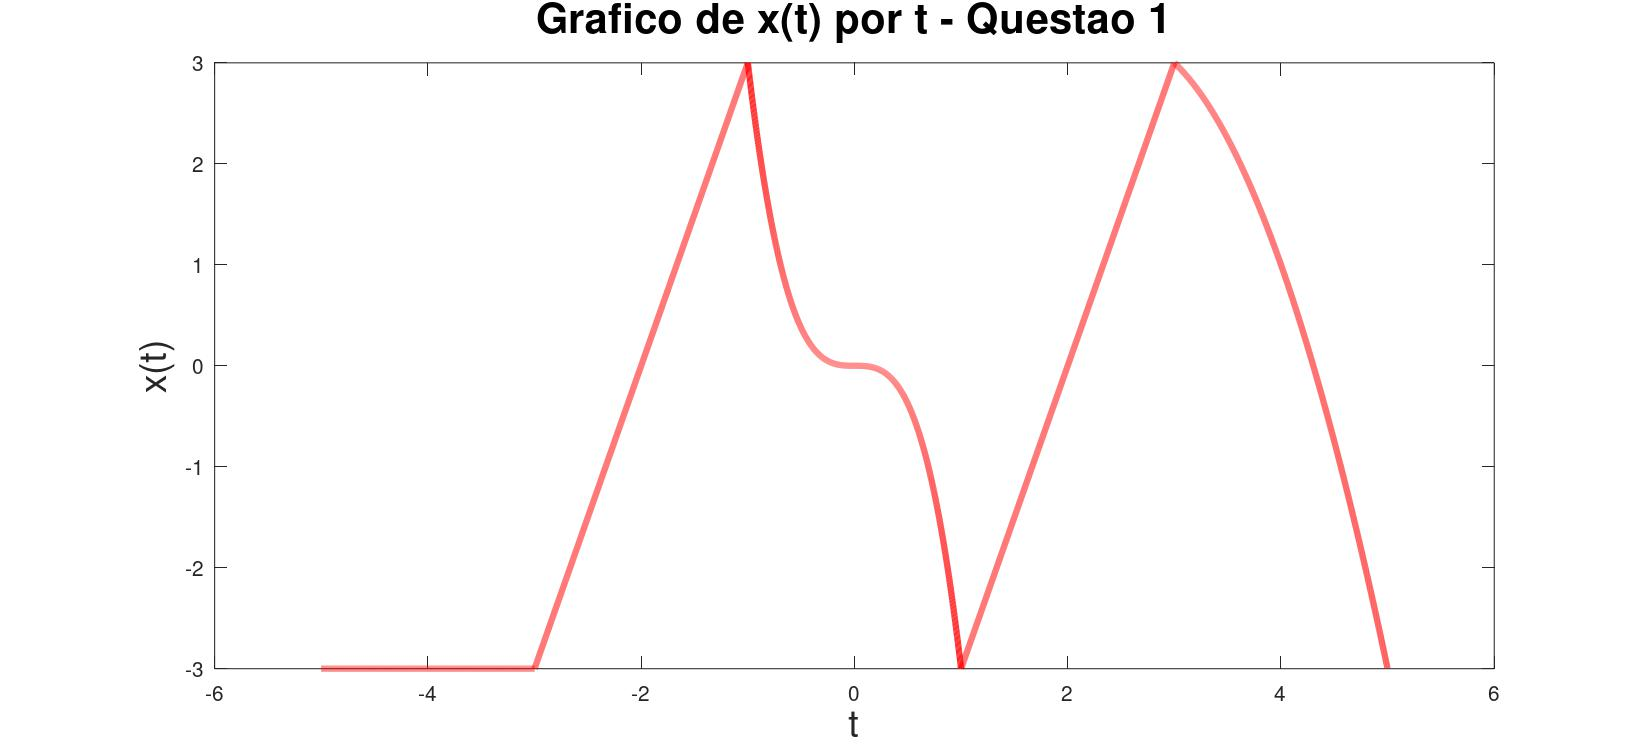
\includegraphics[scale=0.23]{plot1c}
    \centering
\end{figure}

2.) Plotar o gráfico dos sinais a seguir, com escalas adequadas e usando os valores numéricos desejados para os eventuais parâmetros. Dizer se estes sinais são periódicos e, em caso afirmativo quais os seus períodos fundamentais.
(a) $x(t) = sen(\pi t) + cos(2 \pi t) / 2 + sen(3 \pi t) / 3 + cos(4 \pi t) / 4$,
(b) $x(t) = sen(\omega t)cos(50\omega t)$,
(c) $x(t) = sen(\omega t^2)$,
(d) $x(t) = sen(\omega_{1}sen(\omega_{2}t)t)$

\vspace{\baselineskip}

(a) Plotando o gráfico no Octave, temos:

\vspace{\baselineskip}

\begin{figure}[h]
    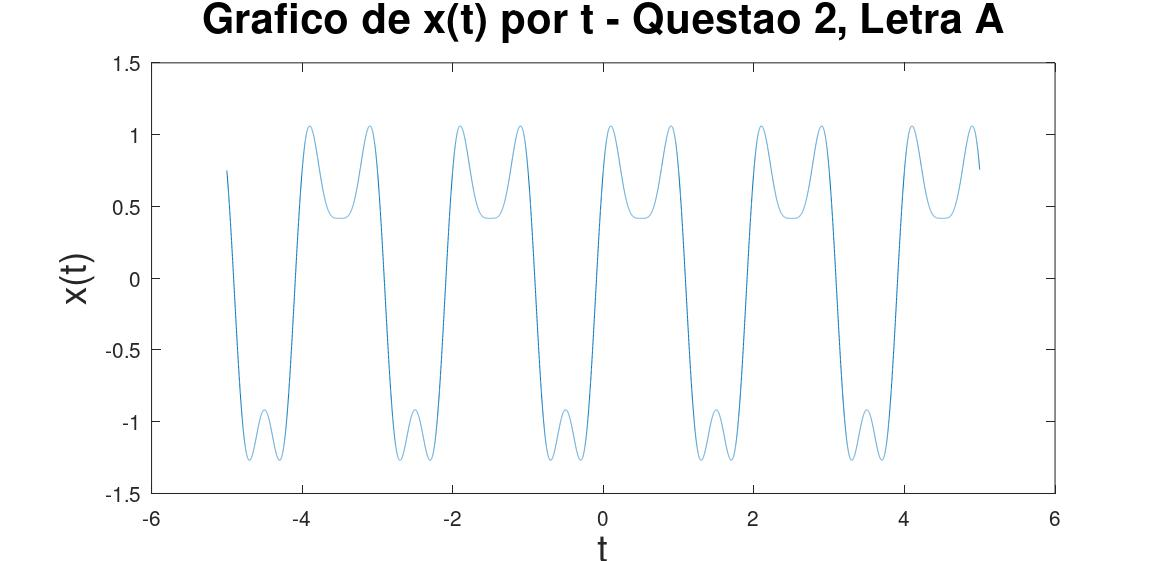
\includegraphics[scale=0.3]{plot2a}
    \centering
\end{figure}

\vspace{\baselineskip}

(b) Plotando o gráfico no Octave, temos:

\vspace{\baselineskip}

\begin{figure}[h]
    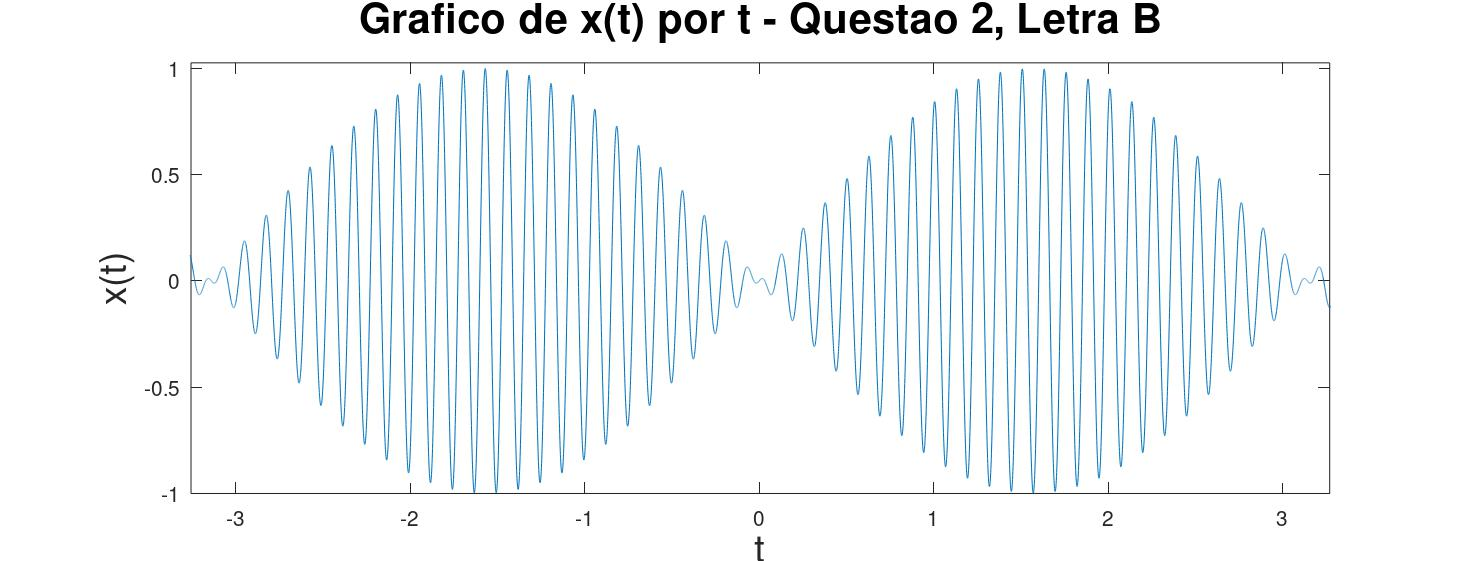
\includegraphics[scale=0.3]{plot2b}
    \centering
\end{figure}

\vspace{\baselineskip}

(c) Plotando o gráfico com o Octave para $\omega = 7$, temos:
\begin{figure}[h]
    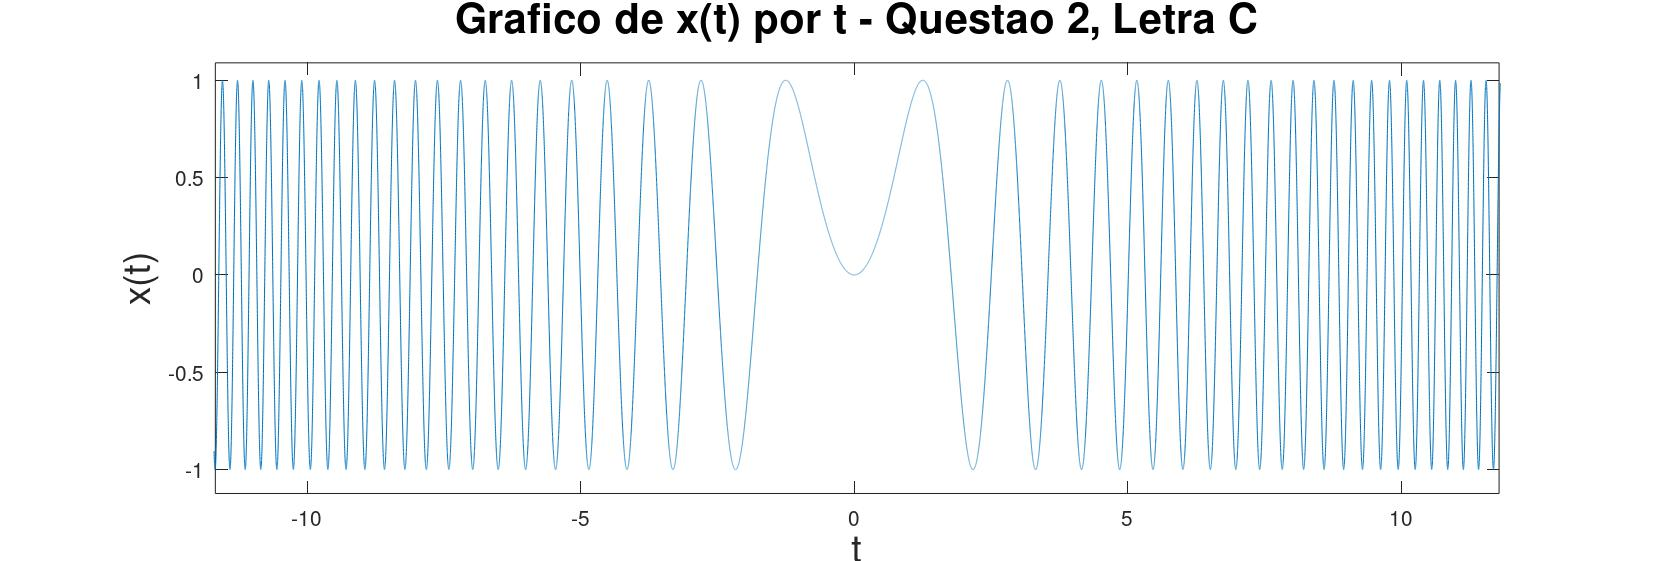
\includegraphics[scale=0.3]{plot2c}
    \centering
\end{figure}

Daqui, já se nota que o sinal não é periódico. Além de ser bem destoante para valores próximos à zero, conforme $t \rightarrow \infty$ ou $t \rightarrow - \infty$, a distância entre as cristas e entre os vales diminui.

\vspace{\baselineskip}

\vspace{\baselineskip}

(d) Plotando o gráfico com o Octave para $\omega_{1} = \omega_{2} = 1$, temos:
\begin{figure}[h]
    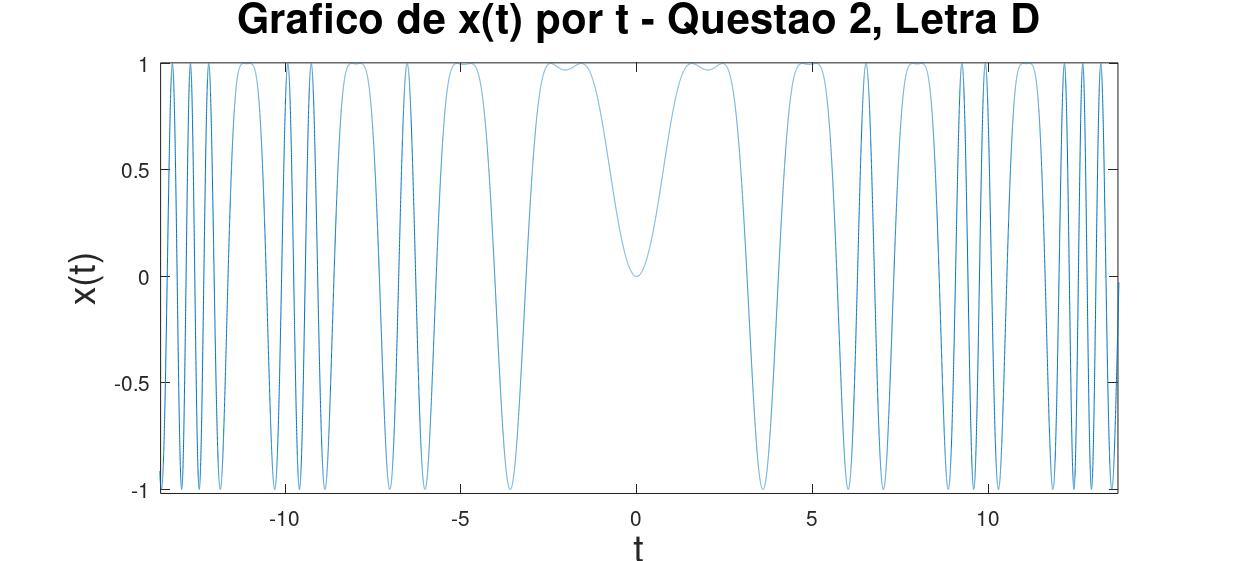
\includegraphics[scale=0.3]{plot2d}
    \centering
\end{figure}

\vspace{\baselineskip}

Do gráfico, nota-se que este sinal não é periódico. As distâncias entre as cristas e entre os vales não é fixa ao longo do gráfico.

\vspace{\baselineskip}

3.) Um sinal periódico com período fundamental $T_{0} = 4 $ é descrito por \textbf{G2}: $x(t) = 1 - e^{|t|}$ para $-T_{0}/2 \leq t < T_{0} / 2$
(a) Esboce o seu gráfico;
(b) calcule analiticamente sua potência total $P$;
(c) calcule $X_{0}$ usando $k = 0$ na fórmula geral de $X_{k}$;
(d) calcule analiticamente os coeficientes $X_{k}$ e verifique se a expressão obtida leva a $X_{0}$ sem indeterminações;
(e) esboce os espectros de módulo e fase;
(f) para $k = 0, 1, 2\;e\;3$, calcule a potência acumulada $P_{k}^{a}$ contida nos harmônicos de $0\;a\;k$;
(g) para $k = 0, 1, 2\;e\;3$, calcule a potência relativa $P_{k}^{a}/P$;
(h) quantos harmônicos são necessários para uma aproximação reter $90.00\%$ da potência?

\vspace{\baselineskip}

4.) O grupo $i$ trabalhará com o sinal periódico $x(t)$ usado pelo grupo $i + 1$ na questão 1 (ao grupo 7: sinal 1). As aproximações numéricas para Octave/MatLab vistas, podem e devem ser utilizadas.
(a) Traçar gráfico;
(b) encontrar potência total $P$;
(c) calcular os $X_{k}$ para $k \in [-10\;10]$;
(d) traçar os espectos de magnitude, fase e potência;
(e) estimar quantos harmônicos são necessários para reter $90.00\%$ da potência;
(f) calcular os coeficientes $a_{k}\;e\;b_{k}$ correspondentes;
(g) traçar, num mesmo gráfico, $x(t)$ e as aproximações.

\vspace{\baselineskip}

5.) Na escala de tempo {\tt t=0:1/2000:5}, considere um sinal de áudio simples $x_{b}(t) = sen(2 \pi f_{0}t)$ ou $x_{b}(t) = cos(2 \pi f_{0}t)$ com frequência \textbf{G2:} $f_{0} = 132Hz$. Ouça este som usando o comando {\tt sound(xb)} no Octave; o resultado é, provavelmente, desagradável pois se trata de uma frequência pura e a sensação é seca, metálica. Para melhorar o \textbf{timbre} do som é preciso colocar mais harmônicos. Crie, na mesma escala de tempo, com a mesma frequência fundamental $f_{0}$, com parâmetros a seu critério e usando até o harmônico $k = 6\;(6f_{0}Hz)$ os sinais a seguir. Ouça cada um deles e compare a qualidade do timbre.\\
(a) Uma onda quadrada $x_{q}(t)$;
(b) uma onda triangular $x_{t}(t)$;
(c) um seno semi-retificado sem o nível DC $x_{s}(t)$;
(d) Opcional: adicionando senos e co-senos harmônicos a seu critério, imagine-se projetando um sintetizador de som e crie um sinal periódico $x(t)$ com frequência fundamental $f_{0}$ e um timbre agradável.


\end{document}
